\documentclass{article}
\usepackage[margin=1in]{geometry}
\usepackage{amsmath, amssymb, amsthm}
\usepackage{enumitem}

% colored links
\usepackage{hyperref}
\hypersetup{
    colorlinks=true,
    linkcolor=blue,
    filecolor=magenta,      
    urlcolor=blue,
    }
% Inputting Python code
\usepackage[dvipsnames]{xcolor}
\definecolor{textblue}{rgb}{.2,.2,.7}
\definecolor{textred}{rgb}{0.54,0,0}
\definecolor{textgreen}{rgb}{0,0.43,0}
\usepackage{upquote}
\usepackage{listings}
\lstset{
    language=Python, 
    tabsize=4,
    basicstyle={\ttfamily},
    keywordstyle=\color{textblue},
    commentstyle=\color{textgreen},
    stringstyle=\color{textred},
    frame=none,
    columns=fullflexible,
    keepspaces=true,
    showstringspaces=false,
    xleftmargin=-15mm, % manual adjustment, figure out permanent solution
}

%Creating algorithms
\usepackage{algorithm}
\usepackage[noend]{algpseudocode}
\usepackage{tcolorbox}

%Images
\usepackage{graphicx}
    \usepackage{subcaption}
    \usepackage{float}
    % \usepackage[labelsep=period]{caption}

%Formatting and Spacing
\setitemize[1]{noitemsep, parsep = 5pt, topsep = 5pt}
\setenumerate[1]{label = (\alph*), parsep = 1pt, topsep = 5pt}
\setlength\parindent{0pt}
\linespread{1.1}

% title
\title{\vspace{-1cm}CS 2051: Honors Discrete Mathematics \\Spring 2023 Homework 3 Supplement}
\author{Sarthak Mohanty}
\date{}

\begin{document}

\maketitle

\section*{Overview}
    With an endless array of ideas, theorems, and algorithms, the field of discrete mathematics can be thought of as a vast museum, filled to the brim with centuries worth of mathematical treasures.. In this supplement, I'll act as your tour guide through this museum, and introduce some of the most impactful problems in recent history, such as the \textbf{Boolean Satisfiability Problem} and the \textbf{Four Color Theorem}. As you journey through these exhibits, you'll also get the chance to curate and contribute something of your own. By utilizing code, you'll be able to add a distinctive and innovative perspective to these important concepts.

\section*{Part 1: Inference (10 pts)}
    As you've seen on your homework this week, rules of inference are difficult to get right. It can often take a lot of time and energy to check if a conclusion is valid. Luckily, by exercising our programming skills, we can expedite this procedure.

    \vspace{3mm}
    \textbf{In this part, you'll implement the following function:}
    \begin{tcolorbox}[colback=blue!10]
        \lstinline{infer(inference_rules, conclusion)}: This function takes in a list of inference rules and a conclusion (both in their string representations), and returns \verb+True+ iff the conclusion can be proved using the provided rules. For example, testing the function on the familiar "modus ponens" rule yields:
        \begin{lstlisting}[belowskip=-10pt]
            >>> infer(["p |implies| q", "p"], "q")
            True
        \end{lstlisting}
    \end{tcolorbox}
    Since you've been acquainted with manipulating propositions of this nature from the last supplement, this method should (hopefully!) not take too long.

\vspace{-1mm}
\section*{Part 2: Satisfiability (10 pts)}
    We continue our exploration of propositional logic with the boolean satisfiability problem, commonly referred to as \verb+SAT+. Let's begin our explanation by informally summarizing \verb+SAT+ with the following story:
    \begin{tcolorbox}[colback=red!10]
        You are in charge of elections for the Georgia Tech Advisory Board. Elections for the board work as follows: there are $n$ candidates, and any number of them, from 0 (nobody) to $n$ (everybody) can be elected as the result of the elections. Each voter provides a list of candidates they want elected and candidates they want not elected. For example, if we call the candidates A, B and C, then one vote might be ``A, B, not C". We say a voter will be satisfied with the results of the election if at least one of his/her preferences is met. For example, the voter with the ``A, B, not C" vote will be satisfied if either A or B is elected, or if C is not elected. Is it possible to choose some combination of people to elect to the board such that everyone is satisfied? 
    \end{tcolorbox}
    Now that you have some semblance of intuition for the problem, let's formalize it using logical notation. Define a \textit{clause} as a disjunction (`$\lor$'ing) of variables or their negations. For example, one such clause would be $(p \lor \neg q_{0} \lor r_{10})$. A proposition is in \textit{conjunctive normal form} (CNF) if it is expressed as a conjunction (`$\land$'ing) of clauses, such as the proposition $(p \lor \neg q_{0}) \land (q_{0} \lor \neg r_{10}) \land (r_{10} \lor \neg p)$. Finally, we say a proposition is \textit{satisfied} by an model if the proposition evaluates to \lstinline{True} under the model. For example, one model satisfying the above proposition is $p = \text{\lstinline{False}}$, $q_{0} = \text{\lstinline{False}}$, $r_{10} = \text{\lstinline{False}}$.

    \vspace{2mm}
    Formally, the \lstinline{SAT} problem asks ``Given a proposition in CNF, is it possible to create a satisfiable model?"

\subsection*{Brute Force Solver}
        One solution to the \lstinline{SAT} problem is simple: generate all possible models for the proposition, and evaluate the function over each of them. This has all been done for you in the function \lstinline{brute_force_SAT_solver}. However, generating all the models is computationally expensive, since for $n$ variables there exist $2^{n}$ possible models. Another way to say this is that the runtime of this function is \textit{exponential}.

\subsection*{WalkSAT Solver}
        For Part 3, we will need a more efficient SAT solver. Luckily, we have many to choose from. In this supplement, we adopt the \lstinline{WalkSAT} algorithm, developed by Christos Papadimitriou.\footnote{Papadimitriou is also the coauthor of the textbook \textit{Algorithms} used in CS 3510.} It's an example of a \textit{randomized} algorithm, an algorithm that uses some degree of randomness as part of its logic. The pseudocode for the algorithm is provided below:
    
    \begin{algorithm}
        \caption{\textsc{WalkSAT}$(prop, p, maxFlips)$}\label{alg:cap}
        \label{alg:walkSAT}
        \begin{algorithmic}
            \State $m =$ randomly chosen assignment to all variables in $prop$
            \For{$flip=1$ \textbf{to} $maxflips$}
                \If {$m$ satisfies $prop$} \Return{$m$} \EndIf
                \State $c = \text{randomly selected unsatisfied clause in $prop$}$
                \State \textbf{with probability} $p$  flip a randomly selected variable in $c$
                \State \textbf{otherwise} flip a variable in $c$ which will result in the fewest previously satisfied clauses to be unsatisfied
            \EndFor
            \State \Return{\lstinline+None+}
        \end{algorithmic}
    \end{algorithm}

    \textbf{In this part, you'll implement the following function:}
    \begin{tcolorbox}[colback=blue!10]
            \lstinline{walkSAT_solver(proposition, p, maxFlips)}: This function takes in a proposition in CNF and outputs a satisfying assignment (or \lstinline{None} if no such assignment exists). Implement this algorithm according to the specifications outlined in Algorithm \ref*{alg:walkSAT}. (Some of the algorithm has already been completed for you, but you must fill in the rest.) The random nature of the algorithm guarantees a solution will eventually be found, but if it takes too long, the \lstinline{maxFlips} parameter should ensure the algorithm is prematurely ended. A successful implementation should output something like:
            \begin{lstlisting}[belowskip=-5pt]
                >>> print(walkSAT_solver('(p or (not q0)) and (q0 or (not r10)) \
                                          and (r10 or (not p))', 0.2, 10000))
                {'p': True, 'q0': True, 'r10': True}
            \end{lstlisting}
            A few tips:
            \begin{itemize}
                \item Use the \lstinline{random.choice()} method to pick a random element from a list. 
                \item An event occurring with probability $p$ can be emulated with \lstinline{random.random() < p}.
            \end{itemize}
    \end{tcolorbox}
    
\section*{Part 3: Reductions (10 pts)}
    We've learned about the \lstinline{SAT} problem, but what's the purpose? The short answer is that many other ``difficult" problems can be represented as an equivalent \lstinline{SAT} problem. One such ``difficult" problem is the four coloring problem, or \lstinline{4COLOR}. As before, we provide an introduction to this problem through an analogy:
    \begin{tcolorbox}[colback=red!10]
        Congrats! You've been elected president of a new country, Britoville. You have four resources you want to be mined throughout the country: rubies, sapphire, emeralds, and gold. For efficiency purposes, you don't want neighboring states mining the same resource. Can you find an assignment of states to resources such that no neighboring states mine the same resource?
    \end{tcolorbox}

    \vspace{2mm}
    Let's formalize this problem as follows: as input, we will take the number of regions $n$, and assume the regions are labeled using numbers 1 to $n$, and a list of neighboring regions of the form ${i,j}$ with $i\neq j$, indicating regions $i$ and $j$ are neighbors. Let us use colors red ($r$), blue ($b$), green ($g$), and yellow ($y$) to color the regions. Our variables are going to be $r_i$, $b_i$, $g_i$ and $y_i$, for $1 \leq i \leq n$, indicating that region $i$ is colored red, blue, green, or yellow, respectively.
    
    \vspace{2mm}
    The \lstinline{4COLOR} problem then asks ``Can a set of regions be colored using at most these four colors such that no two neighbouring regions are coloured the same?" See the addendum \hyperlink{fct}{below} for more information regarding the history of this problem. 

\subsection*{4COLOR to SAT}
    While we don't know how to solve this problem, by converting the \lstinline{4COLOR} problem to an equivalent \lstinline{SAT} problem, we can run our \lstinline{SAT} solver to generate a solution for the \lstinline{4COLOR} problem. The conversion is as follows: for each region $i$,
    \begin{enumerate}[label = \arabic*.]
        \item First, add $(r_i \lor b_i \lor g_i \lor y_i)$ as a clause, ensuring that region $i$ gets at least one color assigned to it. 
        \item Next, for every pair of colors, say $r$ and $b$, add the clause $(\neg r_i \lor \neg b_i)$, effectively making sure that exactly one color is assigned to each region.
        \item Finally, for any two neighboring regions, say $i$ and $j$, and each color, say $r$, add the clause $(\neg r_i \lor \neg r_j)$. This represents the fact that regions $i$ and $j$ cannot both be colored red.
    \end{enumerate}

    \textbf{In this part, you'll implement the following function:}
    \begin{tcolorbox}[colback=blue!10]
        \lstinline{fourColoringtoSAT(neighbors)}: This problem takes in \lstinline{neighbors} (a representation of the \lstinline{4COLOR} problem) and returns an equivalent proposition constructed in CNF using the method outlined above. Make sure to use the variable names \verb+ri+, \verb+bi+, \verb+gi+, and \verb+yi+ to indicate the $i$-th region will be colored red, blue, green, and yellow respectively.
    \end{tcolorbox}

\subsection*{Putting It All Together}
    Finally, it's time to see your hard work come to fruition. In the file \lstinline{fourColor.py}, we've created some methods generating a \href{https://en.wikipedia.org/wiki/Voronoi_diagram}{Voronoi diagram} to help simulate Britoville. An example is shown in Figure (\ref{fig:walkSAT}). If \lstinline{walkSAT_solver} is implemented correctly, running the main function in the file should generate a successful coloring.
    
    \vspace{2mm}
    However, when we set \lstinline{num_points} higher than $\approx 30$, our \lstinline{walkSAT} solver times out, as the coloring problem becomes too large to solve. If you want to generate graphs with more regions, change the \lstinline{solver} parameter in the \lstinline{colormap} call in the main function from \lstinline{walkSAT_solver} to \lstinline{pySAT_solver}. \lstinline{pysat_solver} is a much more powerful solver, and can handle up to 5000 points with ease (for example, the map generated in Figure (\ref{fig:pySAT}) contains 500 points, and was generated in seconds). This solver is also handy if you want to test the \lstinline{fourColoringtoSAT} function without having completed \lstinline{walkSAT_solver}.

    \vspace{-2mm}
    \begin{figure}[H]
        \centering
        \begin{subfigure}{0.49\textwidth}
            \centering
            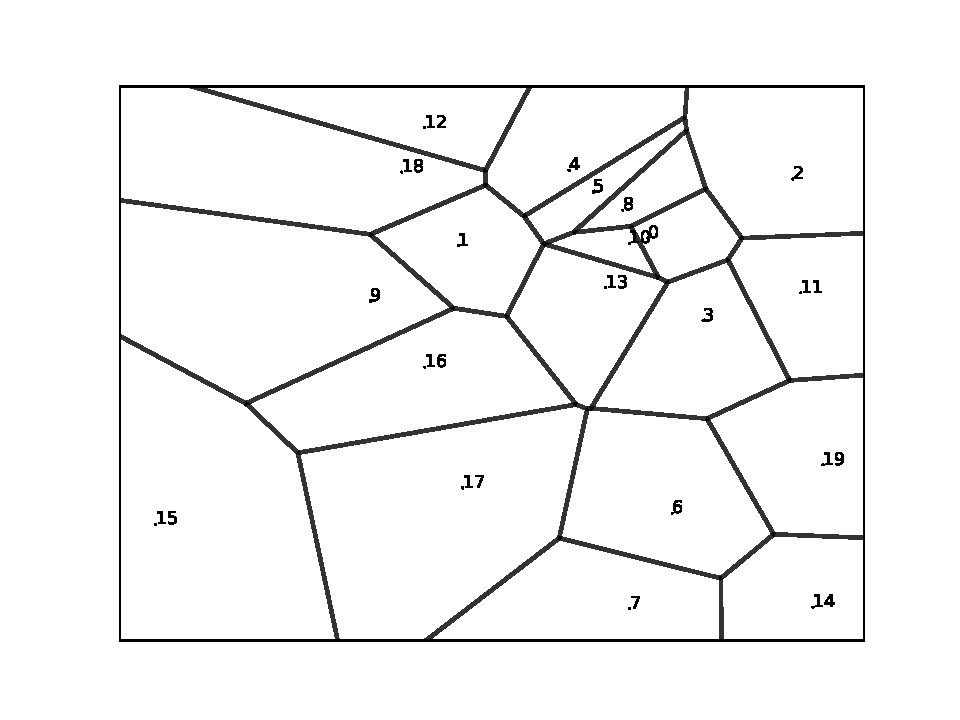
\includegraphics[scale = .5]{sp23/hw-supplements/hw3-supp/images/blank_map.pdf}
        \end{subfigure}
        \begin{subfigure}{0.49\textwidth}
            \centering
            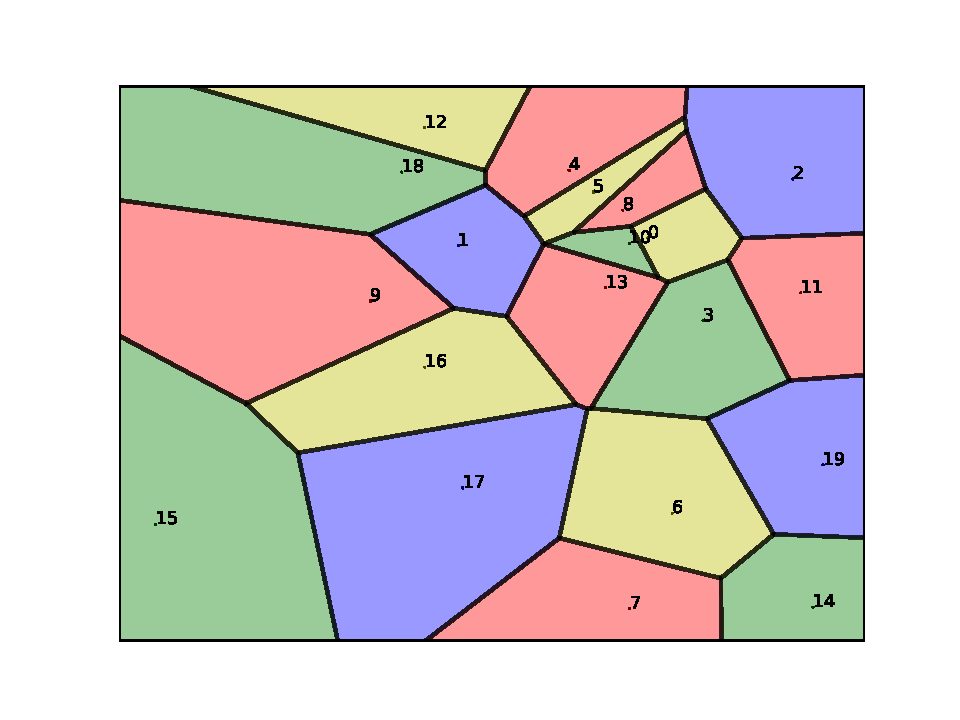
\includegraphics[scale = .5]{sp23/hw-supplements/hw3-supp/images/colored_map.pdf}
        \end{subfigure}
        \caption{A map coloring generated using the \lstinline{walkSAT} solver.}
        \label{fig:walkSAT}
    \end{figure}

    \vspace{-8mm}
    \begin{figure}[H]
        \centering
        \begin{subfigure}{0.49\textwidth}
            \centering
            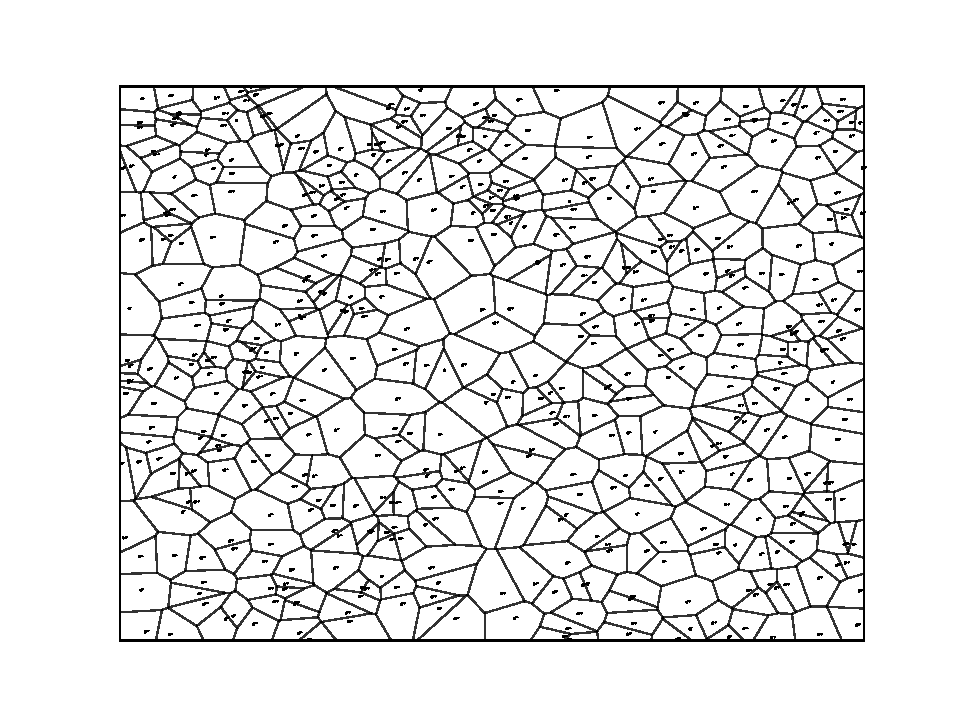
\includegraphics[scale = .5]{sp23/hw-supplements/hw3-supp/images/blank_map2.pdf}
        \end{subfigure}
        \begin{subfigure}{0.49\textwidth}
            \centering
            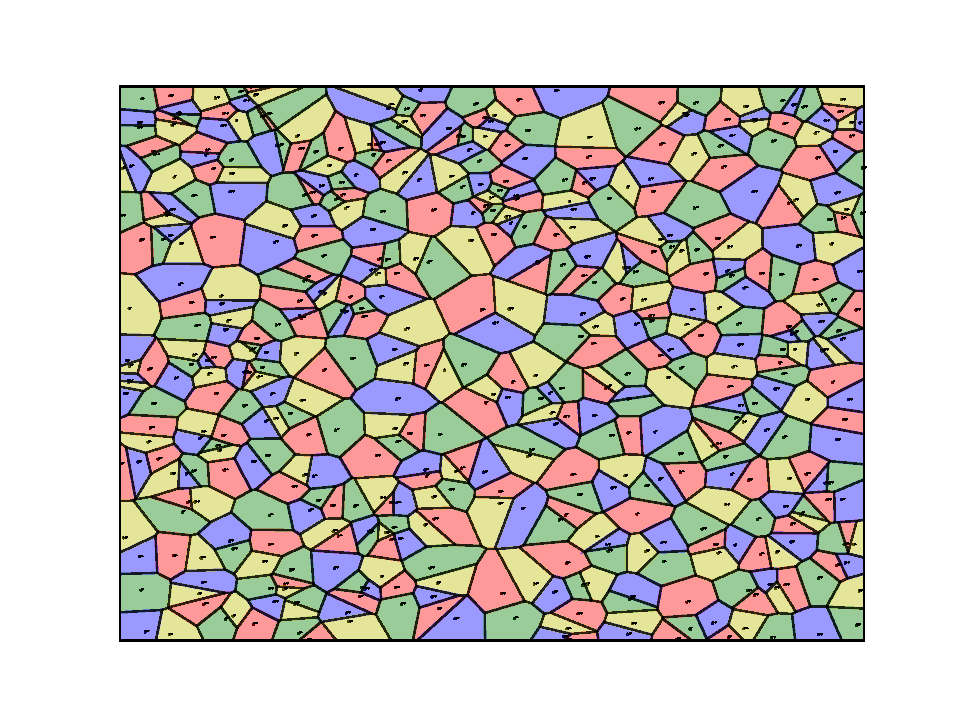
\includegraphics[scale = .5]{sp23/hw-supplements/hw3-supp/images/colored_map2.pdf}
        \end{subfigure}
        \caption{A much larger map coloring generated using the \lstinline{pySAT} solver.}
        \label{fig:pySAT}
    \end{figure}

    \begin{tcolorbox}[colback=green!10, phantom=\phantomsection\hypertarget{fct}]

        \textbf{The Four Color Theorem.}
        The Four Color Theorem claims that the \lstinline{4COLOR} problem is always true; in other words, it states that every (planar) map can be colored using only four colors or less such that no two adjacent regions have the same color. The theorem, first posited in 1852, proved to be a challenging puzzle even for the likes of Augustus De Morgan. (yes, that De Morgan!)

        \vspace{3mm}
        Countless others tried their hand at a proof, but none were successful until 1976, when two mathematicians at the University of Illinois, Kenneth Appel and Wolfgang Haken announced their computer-assisted proof.  It was the first major theorem to be proven with extensive computer assistance, and was initially met with doubt and concern.

        \vspace{3mm}
        It took many years for the proof to gain widespread acceptance, and even now mathematicians approach computer-assisted proofs with trepidation. In fact, some claim that ``proofs” should only be accepted if they are proved by people, not machines, and any work performed by machines should be regarded only as ``calculation." Nevertheless, is of the author's personal opinion that computer-assisted proofs are a definitive step in the right direction.
    \end{tcolorbox}

\section*{Submission Instructions (10 pts)}
    After you fill the appropriate functions, submit the following files to Gradescope and make sure you pass all test cases:
    \begin{itemize}
        \item \lstinline{inference.py}
        \item \lstinline{SAT.py}
        \item \lstinline{fourCOLOR.py}
    \end{itemize}

    \vspace{3mm}
    \textbf{Notes}

    \begin{itemize}
        \item Propositional variables are notated differently as compared to the last supplement. Propositional variables now consist of a letter from \lstinline{[p-z]}, followed by an optional number (ex. \lstinline{p0}, \lstinline{r10}, \lstinline{r200}). This change has been made to help complete Part 3, and should not affect your implementations otherwisee.
        \item The autograder may not reflect your final grade on the assignment. We reserve the right to run additional tests during grading.
        \item Do not import additional packages, as your submission may not pass the test cases.
        \item If you think you may encounter dependency/versioning issues by running code on your local machine, try completing the assignment on \href{https://colab.research.google.com/}{Google Colab}.
    \end{itemize}


\end{document}